\subsection{Lingkaran}

\begin{center}
\begin{tikzpicture}
\coordinate (O) at (0,0);
\coordinate (B) at (0:2cm);
\coordinate (A) at (210:2cm);
\coordinate (D) at (180:2cm);
\coordinate (C) at (130:2cm);
\coordinate (E) at (-20:2cm);

\draw (O) circle (2cm);

\draw (A) -- (B) -- (C) -- (D) -- cycle;
\draw (A) -- (E) -- (C);
\draw[red] (A) -- (C);

\tkzDefPointBy[projection=onto A--C](O) \tkzGetPoint{F}
\draw[orange] (O) -- (F);
\draw[blue] (C) -- (O) -- (A);

\node[right] at (B) {$B$};
\node[below left] at (A) {$A$};
\node[left] at (D) {$D$};
\node[above left] at (C) {$C$};
\node[below right] at (E) {$E$};
\node[right] at (O) {$O$};
\node[above right] at (F) {$F$};
\end{tikzpicture}
\end{center}

    
Misalkan $O$ pusat lingkaran $\Gamma$ dan $A,B,C,D,E$ adalah sembarang titik pada lingkaran $\Gamma$ seperti pada gambar.
\begin{enumerate}
    \item $CO=OA$ adalah jari-jari dengan $\angle ACO = \angle OAC$.
    \item Misalkan titik $F$ adalah titik tengah tali busur $CA$, maka $OF \perp CA$ atau $OF$ tegak lurus dengan $CA$, dengan kata lain, $F$ adalah proyeksi titik $O$ ke $CA$
    \item (Sudut keliling-sudut pusat) Untuk$\angle COA = 2\angle CBA$.
    \item (sudut keliling) $\angle CBA = \angle CEA$.
    \item $ABCD$ adalah segiempat tali busur atau segiempat siklis  atau $A,B,C,D$ terletak di lingkaran (seperti pada gambar) jika dan hanya jika $\angle CBA + \angle ADC = 180^\circ$ atau $\angle ABD = \angle ACD$.
\end{enumerate}

\subsection{Latihan Soal Lingkaran}
\begin{enumerate}
    \item Pada segiempat $WXYZ$ dengan diagonal yang saling tegak lurus diketahui bahwa $\angle WZX = 30^\circ, \angle XWY = 40^\circ,$ and $\angle WYZ = 50^\circ$. Hitunglah besar $\angle X$ dan $\angle Z$.
    \begin{center}
        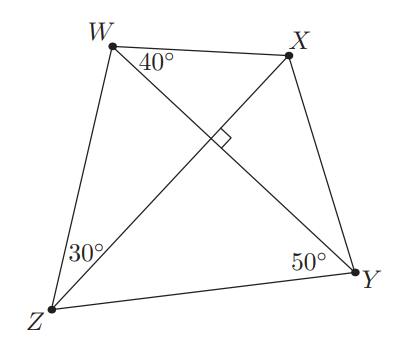
\includegraphics[width=0.25\textwidth]{Soal/Geometry/evanquad.PNG}
    \end{center}
		
    \item (OSK 2013) Diberikan segitiga lancip $ABC$ dengan $O$ sebagai pusat lingkaran luarnya. Misalkan $M$ dan $N$ berturut - turut pertengahan $OA$ dan $BC$. Jika $\angle ABC = 4\angle OMN$ dan $\angle ACB = 6\angle OMN$, maka besarnya $\angle OMN$ sama dengan \dots

    \item 	Pada gambar di bawah, diketahui titik A $\ne$ B pada lingkaran berdiameter $MN$ dan berpusat di $C$. $P$ adalah titik pada segmen $CN$ dimana $\angle CAP = \angle CBP = 10 ^\circ$. Jika $\angle ACM = 40^\circ$, maka $\angle BCN = \dots^\circ$	
    \begin{center}
         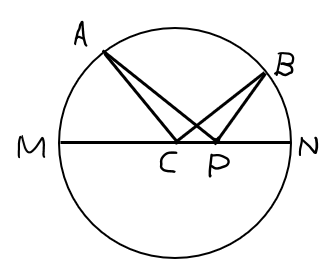
\includegraphics[width=0.25\textwidth]{Soal/Geometry/soalLingkaran1.PNG}
    \end{center}

    \item (OSK 2011,2012,2013,2018) Diberikan segitiga $ABC$ dan lingkaran $\Gamma$ yang berdiameter $AB$. Lingkaran $\Gamma$ memotong sisi $AC$ dan $BC$ berturut-turut di titik $D$ dan $E$. Jika $AD = \frac13 AC, BE =\frac14 BC$ dan $AB = 30$, maka luas segitiga $ABC$ adalah \dots

    \item (OSK 2015) Diberikan segitiga $ABC$ dengan sudut $\angle ABC = 90^\circ$. Lingkaran $L_1$ dengan $AB$ sebagai diameter sedangkan lingkaran $L_2$ dengan $BC$ sebagai diameternya. Kedua lingkaran $L_1$ dan $L_2$ berpotongan di $B$ dan $P$. Jika $AB = 5$, $BC = 12$ dan $BP = x$ maka nilai dari $\frac{240}{x}$ adalah \ldots
\end{enumerate}